\documentclass[a4paper,11pt]{report}


\usepackage[utf8]{inputenc}
\usepackage[T1]{fontenc}
\usepackage{lmodern}
\usepackage[norsk]{babel}
\usepackage{parskip}
\usepackage{graphicx}
\usepackage{caption}
\usepackage{subcaption}
\usepackage{titlepic}
\usepackage{a4wide}
\usepackage{lettrine}
\usepackage[htt]{hyphenat}
\usepackage{enumitem}
\usepackage{color}
\usepackage{hyperref}
\usepackage{listings}
\usepackage[section]{placeins}


%Configuration for lstlistings

\definecolor{lightgray}{rgb}{.9,.9,.9}
\definecolor{darkgray}{rgb}{.4,.4,.4}
\definecolor{purple}{rgb}{0.65, 0.12, 0.82}

\lstdefinelanguage{JavaScript}{
  keywords={typeof, new, true, false, catch, function, return, null, catch, switch, var, if, in, while, do, else, case, break},
  keywordstyle=\color{blue}\bfseries,
  ndkeywords={class, export, boolean, throw, implements, import, this},
  ndkeywordstyle=\color{darkgray}\bfseries,
  identifierstyle=\color{black},
  sensitive=false,
  comment=[l]{//},
  morecomment=[s]{/*}{*/},
  commentstyle=\color{purple}\ttfamily,
  stringstyle=\color{red}\ttfamily,
  morestring=[b]',
  morestring=[b]"
}

\lstset{
   language=JavaScript,
   backgroundcolor=\color{lightgray},
   extendedchars=true,
   basicstyle=\footnotesize\ttfamily,
   showstringspaces=false,
   showspaces=false,
   numbers=left,
   numberstyle=\footnotesize,
   numbersep=9pt,
   tabsize=2,
   breaklines=true,
   showtabs=false,
   captionpos=t
}

\lstdefinestyle{java1}{
  language=Java,
  basicstyle={\ttfamily\footnotesize},
  numberstyle={\ttfamily\footnotesize},
  keywordstyle={\ttfamily\footnotesize\color[rgb]{0,0,1}},
  commentstyle={\ttfamily\footnotesize\color[rgb]{0.133,0.545,0.133}},
  stringstyle={\ttfamily\footnotesize\color[rgb]{0.627,0.126,0.941}},
  breaklines=true,
  columns=fixed,
  extendedchars=true,
  numbers=left,
  numbersep=3pt,
  showspaces=false,
  showstringspaces=false,
  stepnumber=1,
  tabsize=2
}
\lstset{style=java1,
literate=%
{�}{{\ae}}1
{�}{{\aa}}1
{�}{{\o}}1
{�}{{\AE}}1
{�}{{\AA}}1
{�}{{\O}}1
}
\renewcommand\lstlistingname{Eksempel}
\renewcommand\lstlistlistingname{Eksempler}


\usepackage{fancyhdr}
\setlength{\headheight}{15.2pt}
\pagestyle{fancy}
\fancypagestyle{plain}{ %
  \fancyhf{} % remove everything
  \renewcommand{\headrulewidth}{0pt} % remove lines as well
  \renewcommand{\footrulewidth}{0pt}
}

%Her kommer opsett av info for pdf filen
%\pdfinfo{%
%  /Title    (Rapport prosjektoppgave i programutvikling)
%  /Author   ()
%  /Creator  ()
%  /Producer ()
%  /Subject  ()
%  /Keywords ()
%}



\begin{document}
\begin{titlepage}
%\begin{center}
 



\title{
\rule{\linewidth}{0.5mm}
\textsc{\LARGE Applikasjonsutvikling DAVE3600\\ \large Dokumentasjon Mappe 2 (Birthday-o-Matic)}
\rule{\linewidth}{0.5mm}
}


\titlepic{
\includegraphics[width=50mm]{./img/bCake.png}}



\author{\LARGE \textsc{\texttt{Lukas David Larsed}}\\ \\ \LARGE \texttt{s198569}}



\date{\today}



%\end{center} 
\end{titlepage}

\maketitle
%\begin{abstract}
\lettrine[lines=3]{T}{his} is place for an abstract to be.

\end{abstract}

%\input{./tex/om_programmet/om_programmet.tex}
\tableofcontents
\lstlistoflistings
\listoffigures
\listoftables


\chapter{Om applikasjonen}


\begin{itemize}
\item All kode i applikasjonen er på engelsk med hensikt til at denne skal eventuelt kompileres på forskjellige miljøer med ulike typer \"encoding\". 
\item Kompilert med SDK versjon 23: Android 6.0 Marchmallow, Build tools: 23.0.0
\item Mål SDK: API 21: Android 5.0 (Lollipop) Minimal SDK: API 19: Android 4.4 (KitKat)
\item ID for applikasjonen: com.example.s198569.hangman
\item Utviklingsmiljø: Android Tools 1.3.2, Fedora Linux 22 x64
\item Debugging og testing gjennomført på LGE Optimus 2X (P990) med Cyanogenmod Android 4.4.4. Enheten har samme skjermstørrelse som målenhet Samsung Nexus S.
\end{itemize}

\chapter{Bruksanvisning}

\chapter{Arkitektur og struktur}

\chapter{Kode og løsninger}
\chapter{Example chapter}
This chapter i just to state an example create reference about some useful \LaTeX code.

\section{Code}
Check out this cool JavaScript code in \ref{code:handy_javascript}.

\begin{lstlisting}[caption=This is some handy JavaScript code, label=code:handy_javascript]
function getmbidFromURL(){
    var x = 0;
    var param = location.search;
    return param.substring(6);
}
\end{lstlisting}

\section{Images}
Here is a fancy screenshot shown in \ref{fig:example1}.

\begin{figure}[ht]
 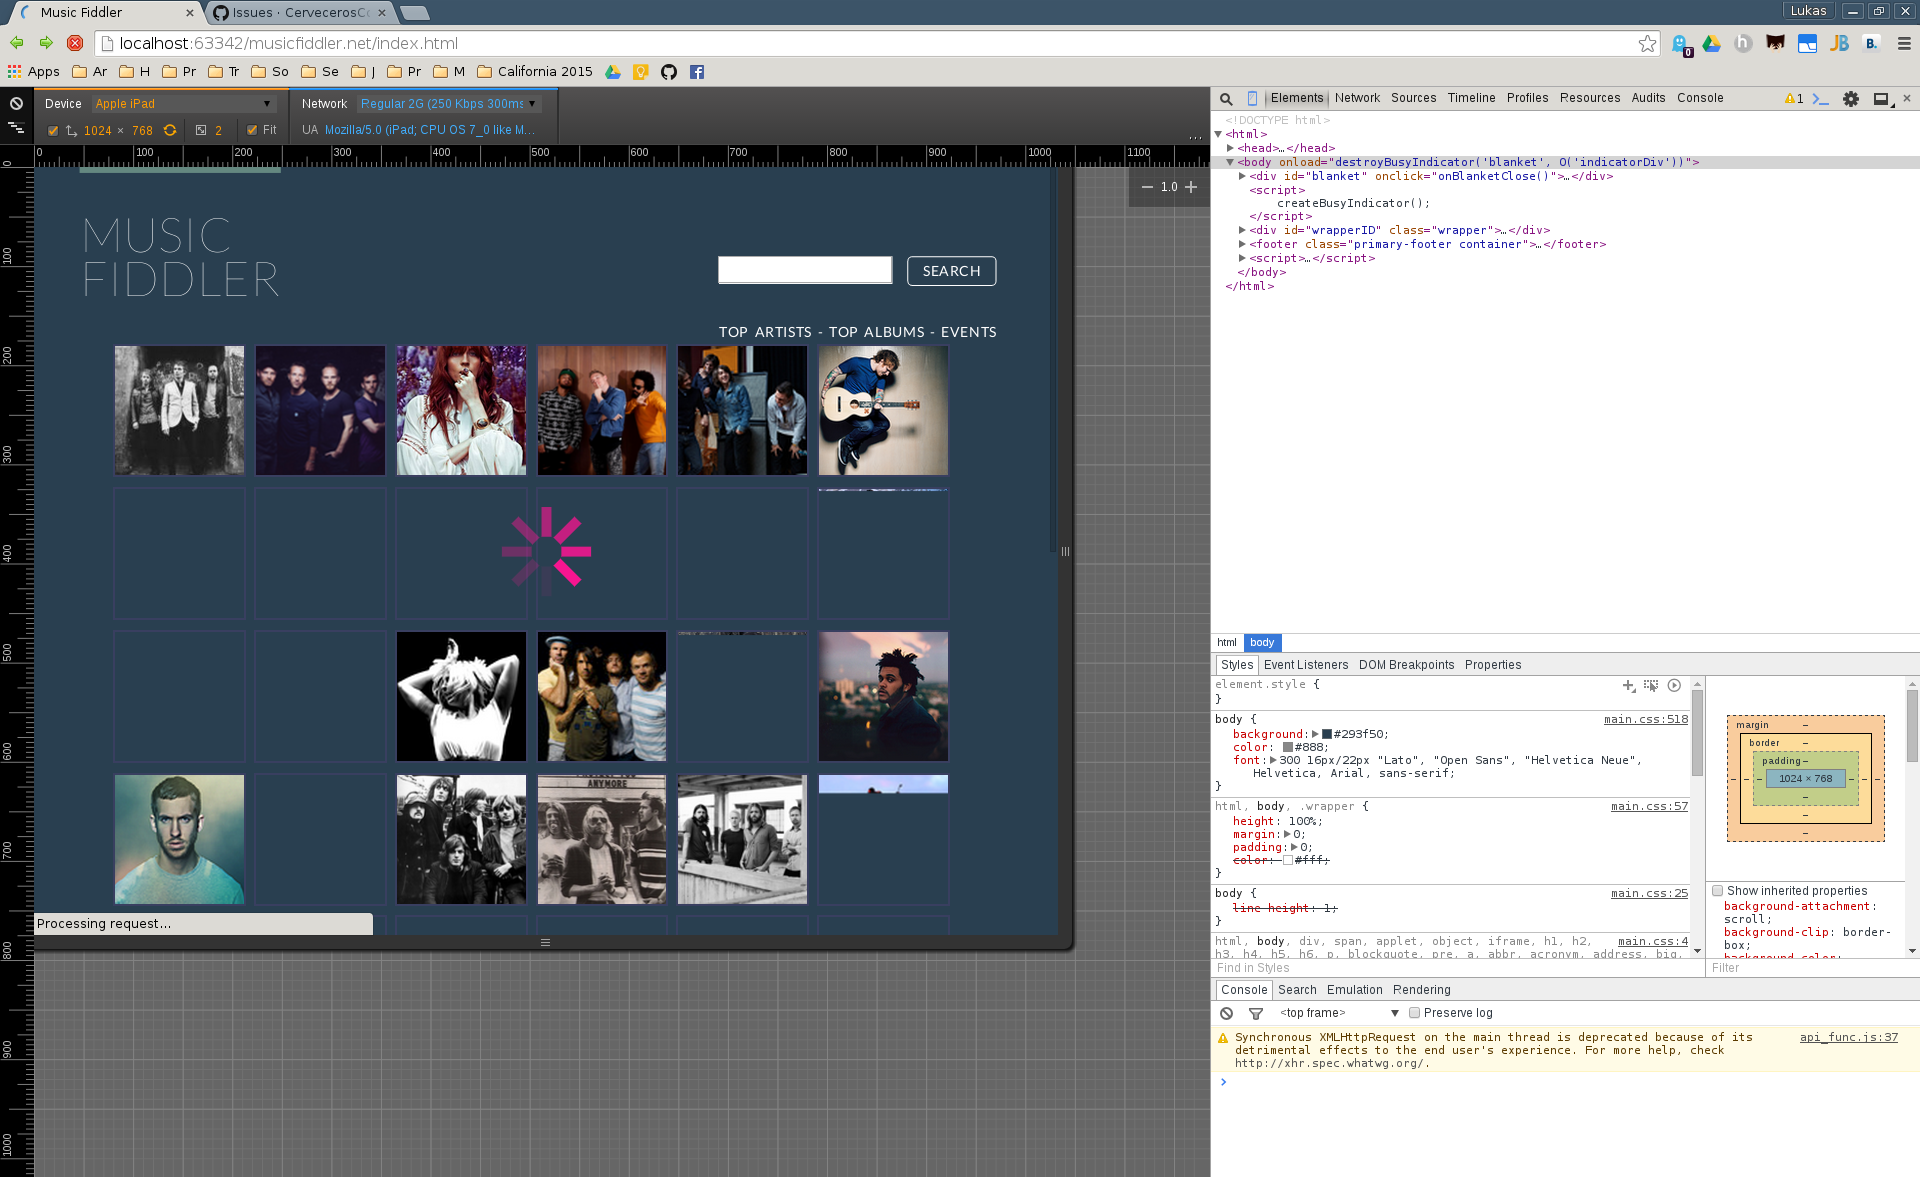
\includegraphics[width=\textwidth,height=\textheight,keepaspectratio]{./img/example/pic1.png}
 \caption[Short caption for table of contents here]{musicfiddler.net in development (this is a place for the long caption)}
 \label{fig:example1}
\end{figure}
%\input{./tex/introduksjon/introduksjon.tex}
%\input{./tex/prosessdokumentasjon/prosessdokumentasjon.tex}
%\input{./tex/produktdokumentasjon/produktdokumentasjon.tex}
%\input{./tex/brukerveiledning/brukerveiledning.tex}
%\input{./tex/testrapport/testrapport.tex}



%Her kommer eksmpler som vi kan bruke n� man skal lage latex i rapporten
%\input{./tex/latex_bruksanvisning/latex_bruksanvisning.tex}

%Appendix for vedlegg og andre ting som ikke direkte passer inn i resten av rapporten
%\input{./tex/appendix/appendix.tex}
\end{document}
